% !TEX encoding = UTF-8 Unicode
\documentclass[fleqn,twoside]{article}
\usepackage[ngerman]{babel}
\usepackage[utf8]{inputenc}
\usepackage[T1]{fontenc}
\usepackage{graphicx}
\usepackage{fancyhdr}
\usepackage{amssymb}
\usepackage{amsmath}
\usepackage{cite}
\usepackage{eurosym}
\usepackage{wrapfig}
\usepackage{tabularx}
\usepackage{pdfpages}
\usepackage{nicefrac}
\usepackage{wasysym}
\usepackage{multirow}
\usepackage{pifont}
\usepackage{textcomp}
\usepackage{comment}
%\usepackage{units}
\usepackage{siunitx}
\usepackage{yfonts}
\usepackage{calligra}
\usepackage{csquotes}
%\usepackage{emerald}
\usepackage{titlesec}
\usepackage{tikz}
\usepackage{stanli}
\usepackage{romanbar}
\usepackage{graphicx}
\usepackage{tabto}
\usepackage{todonotes}
%\usepackage{3dstructuralanalysis}
%\usepackage{structuralanalysis}
\usepackage{enumitem}
\usepackage{booktabs}
\usepackage{float}
\usepackage{siunitx}

%Befehle abändern
%Itemize ohne Lücken
\setlist[itemize]{noitemsep, parsep=0pt, topsep=2pt}
\raggedbottom
%\renewcommand{\todo}[1]{\todo[inline]{#1}}


%Betragsfunktion
\newcommand{\abs}[1]{\ensuremath{\left\vert#1\right\vert}}
%Einheitenfunktion
\newcommand{\un}[2]{{\unit[#1]{\color{black!100}[#2]}}}

\usepackage[pdftex, colorlinks, linkcolor=black, frenchlinks]{hyperref}
\usepackage[a4paper , lmargin = {2.5cm} , rmargin = {2cm} , tmargin = {2.5cm} , bmargin = {2.5cm} ]{geometry}
\pagestyle{fancy}
\setlength{\headheight}{12.51453pt}

\title{\Huge{\textfrak{Angewandte Geotechnik \\Formelsammlung}}}
\author{\calligra{Jonathan C. Walter}\\\calligra{Jonas H. Konrad}}
\date{\textfrak{\today}}

\begin{document}
\parindent 0pt
\fancyhead[L]{Jonathan C. Walter, Jonas H. Konrad}
\fancyfoot[L]{\frakfamily J. C. W.;J. H. K.}
\fancyfoot[R]{\frakfamily }
\fancyfoot[C]{\frakfamily Vor der Hacke ist es duster \\Seite \thepage}
\maketitle \thispagestyle{empty}
%\initfamily %Für Initialien
\begin{center}
FORMELSAMMLUNG NOCH WIRKLICH STARK UNVOLLSTÄNDIG, WIRD IM LAUFE DES WINTERSEMESTERS 22/23 ERWEITERT UND VERVOLLSTÄNDIGT\\
\textfrak{Diese Formelsammlung wurde im Sommersemester 2022 von Jonathan Walter und Jonas Konrad verfasst.\\Kein Anspruch auf Vollständigkeit oder Fehlerfreiheit.\\LaTex Vorlage: github.com/Neowise33}
\end{center}
\tableofcontents
%\listoftodos



\newpage

\section{Allgemeine Formeln}
\begin{itemize}
    \item Spannungsverteilung in Querschnitten: Schneider 4.31
\end{itemize}

%\section{Berechnugsformeln}
\section{Baugruben}

\subsection{Kreisförmiger Grundriss}
\begin{itemize}
    \item Erddruck nach EAB bis $A:B=1,03$ wird ungewollte Asymetrie durch einseitigen Ansatz $p=10$kPa im aktiven oder im Ruhedruck durch: $e_h = p_k \cdot K_h \cdot \cos(\alpha)^2$ berücksichtigt.
    \item Begrenzte Flächen-/Einzellasten belasten 90$^\circ$ des Umfangs.\\ 
    Auf Gegenseite Bettungsreaktiion mit $k_s = \frac{E_s}{R}$
    \item Unmittelbar neben Anfahröffnung keine Bettung ansetzen
\end{itemize}

\subsection{Ovaler Grundriss}
\begin{itemize}
    \item Bis $A:B=1,5$ bzw. $\frac{R_{\text{max}}}{R_{\text{min}}}=2,5$
    \item Nachgiebigkeits-Kategorie 'unnachgiebig' entfällt
    \item Kat.8.8.1 Skript Sonderkonstruktionen
        \begin{table}[H]
        \resizebox{\textwidth}{!}{%
        \begin{tabular}{|l|cc|}
        \hline
        \textbf{Systemnachgiebigkeit} & \multicolumn{1}{c|}{\textbf{Unterer Grenzwert}} & \textbf{Oberer Grenzwert} \\ \hline
        \textbf{Unnachgiebig:} & \multicolumn{1}{c|}{\begin{tabular}[c]{@{}c@{}}$\frac{E_0+E_{aR}}{2}$ \\ nach Walz mit $k_t=1,0$ oder \\ nach Steinfeld mit $\gamma_s=1,0$)\end{tabular}} & $E_0$ wie ebener Fall \\ \hline
        \textbf{\begin{tabular}[c]{@{}l@{}}Annähernd \\ unnachgiebig:\end{tabular}} & \multicolumn{1}{c|}{\begin{tabular}[c]{@{}c@{}}$E_{aR}$ nach Walz/Hock mit $k_t=1,0$ \\ oder Steinfeld mit $\gamma_s=1,0$\end{tabular}} & \begin{tabular}[c]{@{}c@{}}$\frac{E_0+E_{aR}}{2}$ \\ nach Walz mit $k_t=0,5$ oder \\ Steinfeld mit $\gamma_s=0,7$\end{tabular} \\ \hline
        \textbf{Wenig nachgiebig:} & \multicolumn{1}{c|}{$E_a$ nach Beresanzew} & \begin{tabular}[c]{@{}c@{}}$E_{aR}$ \\ nach Walz mit $k_t=0,5$ oder \\ Steinfeld mit $\gamma_s=0,7$\end{tabular} \\ \hline
        \textbf{Nachgiebig:} & \multicolumn{2}{c|}{$E_a$ nach Beresanzew} \\ \hline
        \end{tabular}%
        }
        \end{table}
    
\end{itemize}

\subsection{Hydraulischer Grundbruch bei undurchlässiger Unterwasserbetonsohle}
\begin{itemize}
    \item Vergleich Eigengewicht mit auftreibender Kraft aus Grundwasser:\\ 
    $(G_{Sohle}+G_{Wand})\cdot \gamma_{stb}=(F_{u,Sohle} + F_{u,Wand}) \cdot \gamma_{w}$
        \begin{itemize}
            \item Nach Dicke der Sohle in $F_{u,Sohle}$ auflösen. 
            \item In beiden Auftriebskräften '$F$' nur Tiefe unter Grundwasserspiegel berücksichtigen.
            \item $F_{u,Sohle} = A_{Sohle} \cdot (z_{\text{(OK bis Sohle)}} + d_{Sohle} - z_{GW})\gamma_w$
            \item $F_{u,Wand} = \text{Wanddicke} \cdot U \cdot t_{(\text{Einbindetiefe}-z_{GW})} \cdot \gamma_w$
        \end{itemize}
\end{itemize}

\subsection{Überschnittene Bohrpfahlwand}
\begin{itemize}
    \item Umfang: $U_{\text{Schief}} = (\text{Nettoumdurchmesser} + D_{\text{Bohrpfahl}} + 2 \cdot \text{Schiefstellung} \cdot t_{\text{Höhe}}) \pi$
    \item Gewicht für hydraulischer Grundbruch: $ G_{Wand}= \text{Wanddicke} \cdot U \cdot t_{\text{Höhe}} \cdot \gamma_{Beton}$
    \item Sohlfläche mit Abweichung aus Schiefstellung: Mit $U_{\text{Schief}}$ berechnen
    \item Gewicht Sohle: $G_{\text{Sohle}} = Fd \cdot \gamma_{(UWB)}$
\end{itemize}

\subsection{Theorie}
\begin{itemize}
    \item Schubkraftübertragung Unterwasserbetonsohle:\\
    Sie muss durch Aufwölbung des UWB mobilisiert werden, da die Wand als Druckring trägt und praktisch keinen Auflagerdruck in Radialrichtung auf die Sohle ausübt. Verbesserung der Schubkraftübertragung (zusätzlich zur sorgfältigen Säuberung der Wand durch Taucher) mittels in den Pfählen ausgestemmten ,,Nischen“.
    \item Messtechnische Überwachung einer Baugrube: 
        \begin{itemize}
            \item Fragestellung schädliche Verbauverformungen:
                \begin{itemize}
                    \item Geodätische Vermessung der Verbauwände
                    \item Wandink linometer
                \end{itemize}
            \item Fragestellung schädliche Bodenverformungen:
                \begin{itemize}
                    \item Weitere Vertikalinklinometer im Boden hinter den Wänden
                    \item Setzungsmessungen an GOK
                    \item Evtl. Extensometer parallel zur Ankerrichtung
                \end{itemize}
            \item Fragestellung mögliche Änderungen der Einwirkungen:
                \begin{itemize}
                    \item GW-Beobachtungspegel
                    \item Anker- bzw. Steifenkraftmessung
                \end{itemize}
        \end{itemize}
    \item Gewölbte Sohle: Riskanter als ebene  Ausführung. Zur Sicherheit gegen Fehlstellungen muss die DSV-Sohle dicker ausgeführt werden.
    \item Dafür keine Zugkräfte, dafür Momentengleichgewicht in Sohlmitte mit Eigengewicht, Auftrieb und Moment aus Stich.
    \item Wenn ohne Anker Auftriebskraft über Randreibung übertragen: $V=\frac{B}{2}\cdot (w-d_{Sohle} \cdot \gamma_{Sohle})$
    \item Maximale Reibungskraft: $V = N_{Sohle} \cdot \tan(\varphi)$
\end{itemize}

\subsection{Rückverankerter Unterwasserbeton}
\begin{itemize}
    \item Optimale Pfahllänge $L=A\frac{a^2}{\eta_Z\cdot\gamma_k'}$ und Abstand $a=\frac{B+\sqrt{B^2+4A\cdot C}}{2A}$
    \begin{itemize}
        \item $A=(w_{\min}\cdot \gamma_G+(w_{\max}-w_{\min})\gamma_Q-\gamma_{platte,k}\cdot d_{platte}\cdot \gamma_{G,inf})\frac{\gamma_{s,t\cdot\eta_Z}\cdot\gamma_k'}{U\cdot q_{s,k}}$
        \item $B=\frac{\sqrt{2}}{3}\cot(\varphi_k)\cdot\eta_Z\cdot\gamma_k'$
        \item $C=w_{\min}\frac{\gamma_{G,dst}}{\gamma_{G,stb}}+(w_{\max}-w_{\min})\frac{\gamma_{Q,dst}}{\gamma_{G,stb}}-\gamma_{platte,k}\cdot d_{platte}$
        \begin{itemize}
            \item $\eta_Z=0,8$
            \item $U$: Umfang
            \item $w_{\min}$: kleinster (durchschnittlicher) Wasserdruck
            \item $w_{\max}$: höchster Wasserdruck
        \end{itemize}
    \end{itemize}
\end{itemize}



\section{Bodenbewehrung mit Geokunststoffen}

\subsection{Dämme auf weichem Untergrund}

\begin{itemize}
    \item Nachweis der inneren Standsicherheit ohne Umschlag $E_{ah,d}\le R_{O,d}$ und $E_{ah,d}\le R_{U,d}+\min(R_{B,d};R_{Al,d};R_{AR,d})$
    \begin{itemize}
        \item $E_{ah,d}=\gamma_G\left(\frac{h_1^2}{2}\gamma_{1,k}K_{agh}\right)+\gamma_Q(p_kh_1K_{agh})$
        \item $R_{O,d}=\frac{h_1^2}{2\tan(\beta)}\cdot\gamma_{1,d}\cdot f_{1g,d}$
        \item $R_{U,d}=c_{u2,d}\cdot\frac{h_1}{\tan(\beta)}$ (Undaräniert)\\
        $R_{U,d}=c'_{u2,d}\cdot\frac{h_1}{\tan(\beta)}+\frac{h_1^2}{2\tan(\beta)}\cdot\gamma_{1,d}\cdot f_{2g,d}$ (Dräniert)
    \end{itemize}
    \item Nachweise der inneren Standsicherheit mit einfachem Umschlag $E_{ah,d}\le R_{O,d}+R_{3,d}$ und $E_{ah3,d}\le R_{3,d}$
    \begin{itemize}
        \item $R_{3,d}=\frac{h_3^2}{2\tan(\beta)}\,\gamma_{1,d}\,f_{1g,d}$
        \item $E_{ah3,d}=\gamma_g\left(\frac{h_3^2}{2}\gamma_{1,k}\,K_{agh}\right)+\gamma_Q\,(p_k\,h_3\,K_{agh})$
    \end{itemize}
    \item Nachweise der inneren Standsicherheit gegen ausquetschen $E_{ah4,d}\le R_{Ep4,d}+R_{U,d}+R_{4,d}$
    \begin{itemize}
        \item $E_{ah4,d}=\gamma_G\left(h_1\cdot h_4\cdot \gamma_{1,k}+\frac{h_4^2}{2}\cdot \gamma_{2,k}-2c_{u2,k}\cdot h_4\right)$
        \item $R_{Ep4,d}=\frac{h_4^2}{2}\cdot\gamma_{2,d}+2c_{u2,d}\cdot h_4$
        \item $R_{4,d}=c_{u2,d}\cdot\frac{h_1}{\tan(\beta)}$
        \item $R_{U,d}=\min(R_{B,d};R_{A,d})$
    \end{itemize}
\end{itemize}

\section{Böschungssicherung}

\subsection{Bodenvernagelung}
\begin{itemize}
    \item{Grundlegende Eigenschaften:}
    \begin{itemize}
        \item \textbf{Schubkraftverteilung in den Bewehrungselementen:} \\Herausziehwiderstand/lfm hinter Gleitfläche etwa konstant
        \item \textbf{Mögliche Verschlechterung des Hangmaterials (Verlust der Kohäsion):} \\Kohäsion nicht ansetzen
        \item \textbf{Hangwassereinfluss:} \\Verstopfen von Dränagen
        \item \textbf{Dauerbeständigkeit:} \\doppelter Koressionsschutz nötig
        \item \textbf{Verkehrserschütterung:} \\kein Problem
        \item \textbf{Mögliche Setzungsschäden an Nachbarbauwerken:} \\Bohrauflockerung, größeres Bauwerk und damit näher
    \end{itemize}
\end{itemize}


\subsection{Geokunststoffwand}
\begin{itemize}
    \item{Grundlegende Eigenschaften:}
    \begin{itemize}
        \item \textbf{Mögliche Verschlechterung des Hangmaterials (Verlust der Kohäsion):} \\Im Endzustand nicht relevant
        \item \textbf{Hangwassereinfluss:} \\Schüttung drainiert selbst
        \item \textbf{Dauerbeständigkeit:} \\hohe Abmiderungsfaktoren anzusetzen
        \item \textbf{Verkehrserschütterung:} \\Sackung möglich, Abminderung Kennwerte
        \item \textbf{Mögliche Setzungsschäden an Nachbarbauwerken:} \\keine
        \item \textbf{Schubkraftverteilung in den Bewehrungselementen:} \\Herausziehwiderstand/$m^2$ proportional zur Überlagerung, also Tiefenlage
    \end{itemize}
\end{itemize}

\section{Pfähle}

\subsection{Laterale Pfahlbelastung}

\subsubsection{Elastische Bettung}

\begin{itemize}
    \item Pfahlprobebelastung:\\
        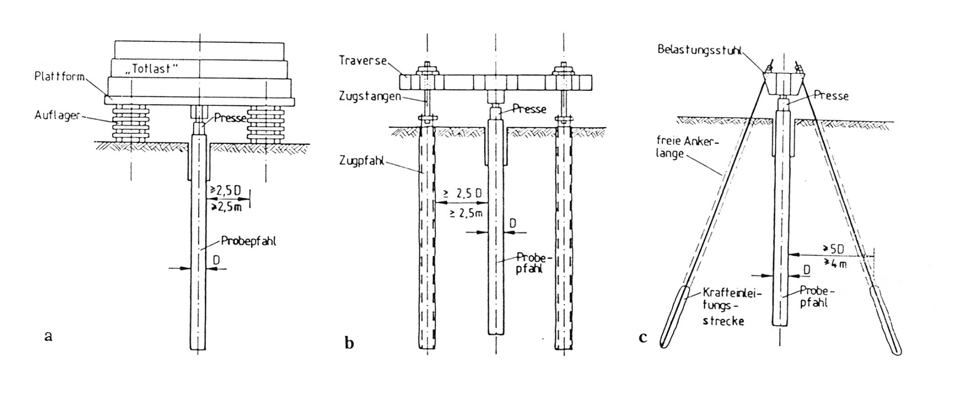
\includegraphics[width=0.99\textwidth]{Grafiken/Pfahlprobebelastung.png}
    \item Ohne Bettungszunahme mit der Tiefe
    \begin{itemize}
        \item Elastische Länge: $L=\sqrt[4]{\frac{4EI}{k_s\cdot D_s}}$
        \item $\lambda=\frac lL$ $\lambda>5$ schlank; $1<\lambda<5$: gedrungen; $0<\lambda<1$: starr
        \item $l$: Tatsächlische Pfahllänge
        \item $x(0)$: Pfahlkopfverschiebung
        \item $\phi(0)$: Pfahlkopfverdrehung
        \item $H$: Horizontalkraft
        \item $D_s$: Pfahldicke
        \item $k_s$: Bettungsziffer
        \item $M_0$: Moment am Pfahlkopf
        \item Gedrungener Pfahl, gelenkig gelagert, Horizontalkraft
        \begin{itemize}
            \item $x(0)=\frac{2H}{k_s\cdot D_s\cdot L}\left(\frac{\sinh(\lambda)\cdot\cosh(\lambda)-\sin(\lambda)\cdot\cos(\lambda)}{\sinh(\lambda)^2-\sin(\lambda)^2}\right)$
            \item $\phi(0)=\frac{2H}{k_s\cdot D_s\cdot L^2}\left(\frac{\sinh(\lambda)^2+\sin(\lambda)^2}{\sinh(\lambda)^2-\sin(\lambda)^2}\right)$
        \end{itemize}
        \item Gedrungener Pfahl, gelenkig gelagert, Kopfmoment
        \begin{itemize}
            \item $x(0)=\frac{2M_0}{k_s\cdot D_s\cdot L^2}\left(\frac{\sinh(\lambda)^2+\sin(\lambda)^2}{\sinh(\lambda)^2-\sin(\lambda)^2}\right)$
            \item $x(0)=\frac{4M_0}{k_s\cdot D_s\cdot L^3}\left(\frac{\sinh(\lambda)\cdot\cosh(\lambda)+\sin(\lambda)\cdot\cos(\lambda)}{\sinh(\lambda)^2-\sin(\lambda)^2}\right)$
        \end{itemize}
        \item Gedrungener Pfahl, Einspannung, Horizontalkraft
        \begin{itemize}
            \item $x(0)=\frac{H}{k_s\cdot D_s\cdot L}\left(\frac{\cosh(\lambda)^2+\cos(\lambda)^2}{\sinh(\lambda)\cdot\cosh(\lambda)-\sin(\lambda)\cdot\cos(\lambda)}\right)$
            \item $M(0)=\frac{-H\cdot L}{2}\left(\frac{\cosh(\lambda)^2+\cos(\lambda)^2}{\sinh(\lambda)\cdot\cosh(\lambda)-\sin(\lambda)\cdot\cos(\lambda)}\right)$
        \end{itemize}
        \item Ideal schlanker Pfahl, gelenkig gelagert, Horizontalkraft
        \begin{itemize}
            \item $x(0)=\frac{2H}{k_s\cdot D_s\cdot L}$
            \item $\phi(0)=\frac{2H}{k_s\cdot D_s\cdot L^2}$
        \end{itemize}
        \item Ideal schlanker Pfahl, gelenkig gelagert, Kopfmoment
        \begin{itemize}
            \item $x(0)=\frac{2M_0}{k_s\cdot D_s\cdot L^2}$
            \item $\phi(0)=\frac{4M_0}{k_s\cdot D_s\cdot L^3}$
        \end{itemize}
        \item Ideal schlanker Pfahl, gelenkig gelagert, eingespannt
        \begin{itemize}
            \item $x(0)=\frac{H}{k_s\cdot D_s\cdot L}$
            \item $\phi(0)=0$
        \end{itemize}
        \item Ideal starrer Pfahl, gelenkig gelagert, Horizontalkraft
        \begin{itemize}
            \item $x(0)=\frac{4H}{k_s\cdot D_s\cdot l}$
            \item $\phi(0)=\frac{6H}{k_s\cdot D_s\cdot l^2}$
        \end{itemize}
        \item Ideal starrer Pfahl, gelenkig gelagert, Kopfmoment
        \begin{itemize}
            \item $x(0)=\frac{6M_0}{k_s\cdot D_s\cdot l^2}$
            \item $\phi(0)=\frac{12M_0}{k_s\cdot D_s\cdot l^3}$
        \end{itemize}
        \item Ideal starrer Pfahl, Eingespannt, Horizontalkraft
        \begin{itemize}
            \item $x(0)=\frac{H}{k_s\cdot D_s\cdot l}$
            \item $\phi(0)=0$
        \end{itemize}
    \end{itemize}
    \item Mit Bettungszunahme mit der Tiefe
    \begin{itemize}
        \item Schlanker Pfahl gelenkig gelagert, Horizontalkraft
        \begin{itemize}
            \item $x(0)=2,4\frac{H}{k_R\cdot L^2}$
            \item $\phi(0)=1,6\frac{H}{k_R\cdot L^3}$
            \item $\max M=0,77H\cdot L$
        \end{itemize}
        \item Schlanker Pfahl gelenkig gelagert, Kopfmoment
        \begin{itemize}
            \item $x(0)=1,6\frac{M_0}{k_R\cdot L^3}$
            \item $\phi(0)=1,74\frac{M_0}{k_R\cdot L^4}$
        \end{itemize}
        \item Schlanker Pfahl eingespannt, Horizontalkraft
        \begin{itemize}
            \item $x(0)=0,93\frac{H}{k_R\cdot L^2}$
            \item $\max M=0,93\cdot H\cdot L$
        \end{itemize}
        \item Ideal starrer Pfahl gelenkig gelagert Horizontalkraft
        \begin{itemize}
            \item $x(0)=18\frac{H}{k_R\cdot l^2}$
            \item $x(0)=24\frac{H}{k_R\cdot l^3}$
            \item $\max M=0,26\cdot H\cdot L$
        \end{itemize}
        \item Ideal starrer Pfahl gelenkig gelagert Kopfmoment
        \begin{itemize}
            \item $x(0)=24\frac{M_0}{k_R\cdot l^3}$
            \item $\phi(0)=36\frac{M_0}{k_R\cdot l^4}$
            \item $\max Q=1,778\frac{M_0}{l}$
        \end{itemize}
        \item Ideal starrer Pfahl eingespannt, Horizontalkraft
        \begin{itemize}
            \item $x(0)=2\frac{H}{k_R\cdot l^2}$
            \item $\max M=0,667\cdot H\cdot l$
        \end{itemize}
    \end{itemize}
\end{itemize}

\subsubsection{Anprall am Pfahlkopf}
\begin{itemize}
    \item Annahme: Linear elastische Pfahlbettung mit Ersatzfeder $H'=C\cdot x_o$
    \item Ideal schlanke Pfähle: $C=\frac12k_s \cdot D\cdot L$
    \item $w_{kin}=\frac12 m\cdot v^2=\int C\cdot x_0\,\text{d}x_0=\frac12C\cdot x_0^2$
\end{itemize}

\subsubsection{Bettungskraft aus Pfahlauslenkung}
\begin{itemize}
    \item Bettungskraft in jeder Tiefe: $p=k_s \cdot x \cdot D$
    \item Auslenkung: $x= \frac{2\cdot H}{k_s \cdot D \cdot L} \cdot \exp(-\frac{Z}{L})\cdot\cos(\frac{Z}{L})$
    \item Charakteristische Bettungskraft: $p=\frac{2\cdot H}{L} \cdot \exp(-\frac{Z}{L}) \cdot \cos(\frac{Z}{L})$
\end{itemize}

\subsubsection{Hangverdübelung}
\begin{itemize}
    \item $\frac{\Delta \tau_k}{\tau_k} = I_v ln(\frac{v_0}{v_1})$
    \item $v_o$ = Ausgangsgeschwindigkeit ; $v_1$ = Endgeschwindigkeit
    \item $\tau_k = \gamma \cdot h_G \sin(\beta) \cos(\beta)$
    \item Schubspannung die von $n$ Dübeln übernommen wird $\ln\left(\frac{v_o}{v_1}\right)$ aus dem Diagramm ablesen: $\Delta \tau_k = \tau_k \cdot I_v \cdot \ln(\frac{v_0}{v_1}) = \frac{Q_{ges,k}}{a\cdot b} = \frac{n \cdot Q_{s,k}}{a \cdot b}$
    \item Von einem Dübelpfahl übernommene Querkraft: $Q_{s,k} = EI \cdot \frac{w}{L^3} \cdot q \left( \frac{h_0}{L} , \frac{h_0}{h_u}\right)$ ; 
    \begin{itemize}
        \item $L = \sqrt[4]{\dfrac{4\cdot EI}{k_{s,k} D_s}}$ ; $k_{s,k} = \frac{E_{s,k}}{D_s}$
        \item $h_0/L$ $h_0/h_u$ aus Diagramm
    \end{itemize}
    
    \item $w_1 = \frac{t_1 \cdot v_0}{\frac{v_0}{v_1}-1} \cdot \ln \left( \frac{v_0}{v_1} \right)$
    \item $t_1 = \frac{a \cdot b \cdot \tau_k \cdot I_v \cdot L^3}{n \cdot EI \cdot q \cdot v_0} \left( \frac{v_0}{v_1} -1 \right)$ ; $t_1$ = Betrachtungszeitraum ; $w_1$ = Kriechmaß
    \item $n = \frac{\Delta \tau_k \cdot a \cdot b}{Q_{s,k \cdot \cos(\beta)}}$
    \item Abstand Dübel quer zur Kriechrichtung: $a_{quer,max} = \frac{2a}{\left( \frac{a}{h_G} +1 \right)}$
    \item $M_{max,k} = EI \cdot \frac{w}{L^2} \cdot m \left( \frac{h_0}{L},\frac{h_0}{h_u} \right)$
    \item Querkraft Dübel:\\
    \includegraphics[width=0.8\textwidth]{Grafiken/Querkraft_Dübel.png}
    \item Moment Dübel:\\
    \includegraphics[width=0.8\textwidth]{Grafiken/Moment_Dübel.png}

    \item Versagen des Bodens in der Pfahlumgebung:
        \begin{itemize}
            \item $E_{1,d} = Q_{s,k} \cdot \gamma_G$
            \item $R_{ph,k} = \gamma \cdot \frac{(h_G^2 - (h_G-h_0)^2)}{2} K_{ph} D_{s}$
            \item $E_{1,d} < R_{1,d} = \frac{R_{ph,k}}{\gamma_{R}}$
        \end{itemize}
    \item Nachweis Materialversagen des Dübelpfahls:
        \begin{itemize}
            \item Durchführen mit: $E_{1,d}$ \& $M_{1,d} = M_{max,k} \cdot \gamma_{G}$ 
        \end{itemize}
    
\end{itemize}

\subsection{Pfahlgruppen}

\subsubsection{Vertikale- und Momentenbelastung von Pfahlgruppen}
\begin{minipage}{0.58\textwidth}
\begin{itemize}
    \item Moment um die $x$-Achse $E_d=\frac{V}{n_x\cdot n_y}\pm \frac{M_x\cdot y_2}{n_x\cdot \sum(y_i)^2}$
    \item Moment um die $y$-Achse $E_d=\frac{V}{n_x\cdot n_y}\pm \frac{M_y\cdot x_2}{n_x\cdot \sum(x_i)^2}$
\end{itemize}
\end{minipage}
\begin{minipage}{0.4 \textwidth}
\begin{tikzpicture}[scale=0.4]
    \foreach \x in {2,5,8}
    \foreach \y in {2,5,8,11}
{   
\draw (0,0) rectangle (10,13);
\draw (\x,\y) circle [radius=1];
}
\draw (0,6.5) -- (12,6.5);
\draw[|-|] (11,6.5) -- (11,8);
\draw[|-|] (12,6.5) -- (12,11);
\draw (10.5,7) node {$y_1$};
\draw (11.5,9) node {$y_2$};
\draw[<->] (5,5) to [bend left] (5,8);
\draw[<->] (5.5,5) -- (5.5,8);

\end{tikzpicture}
\end{minipage}

\subsubsection{Querbelastung von Pfahlgrupppen}
\begin{minipage}{0.58\textwidth}
\begin{itemize}
    \item Gleiche Pfahlverschiebung durch Kopfplatte erzwungen
    \item Unterschiedlicher Bettungsmodul $k_s$ je nach Pfahlstellung
    Gesamtbeanspruchung $H$ verteilt sich ungleichmäßig auf die Pfähle: $\frac{H_i}{H}=\frac{\alpha_i}{\sum\alpha_i}=\frac{\alpha_{Li}\cdot\alpha_{Qi}}{\sum(\alpha_{Li\cdot\alpha_Qi})}$
    \begin{itemize}
        \item $\alpha_L=0,125\left(\frac{a_L}{D}\right)+0,25$ für $2\le\frac{a_L}{D}\le6$
        \item $\alpha_{QA}=0,1\left(\frac{a_Q}{D}\right)$
        \item $\alpha_L=0,25\left(\frac{a_Q}{D}\right)+0,25$ für $2\le\frac{a_Q}{D}\le3$
        \item $k_{si}=k_{s,E}\cdot\left\{\begin{array}{cc}
           \alpha_1^{\frac43}:  &\lambda_E\ge4  \\
            \alpha_i: & \lambda_E \le2
        \end{array} \right.$
    \end{itemize}
\end{itemize}
\end{minipage}
\begin{minipage}{0.4\textwidth}
    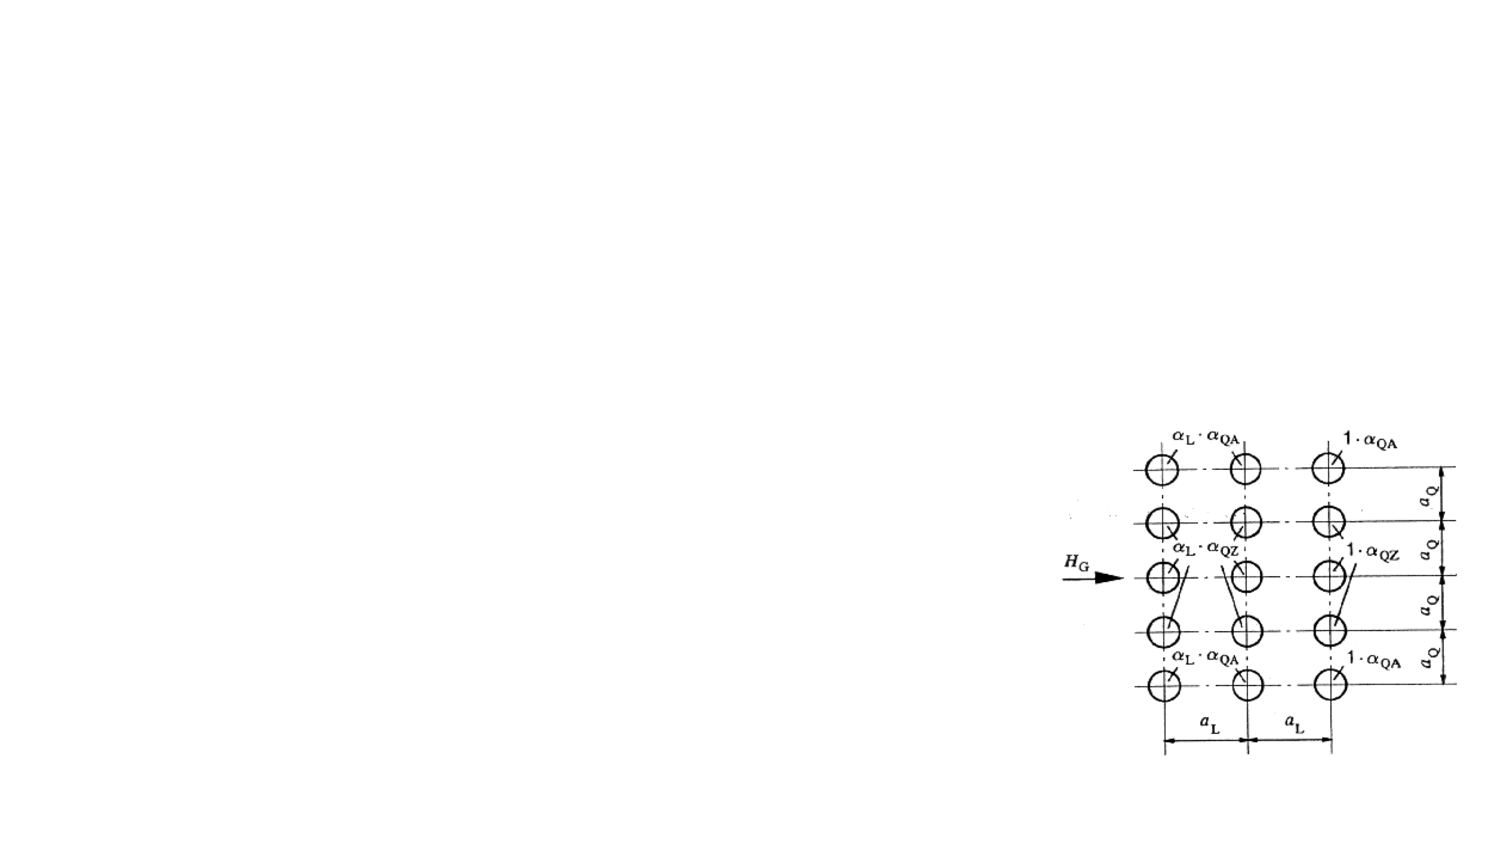
\includegraphics[width=0.8\textwidth]{Grafiken/Pfahlgruppe_Lateral.pdf}
\end{minipage}
\subsubsection{Verfahren für rotationssymetrische Pfahlroste}
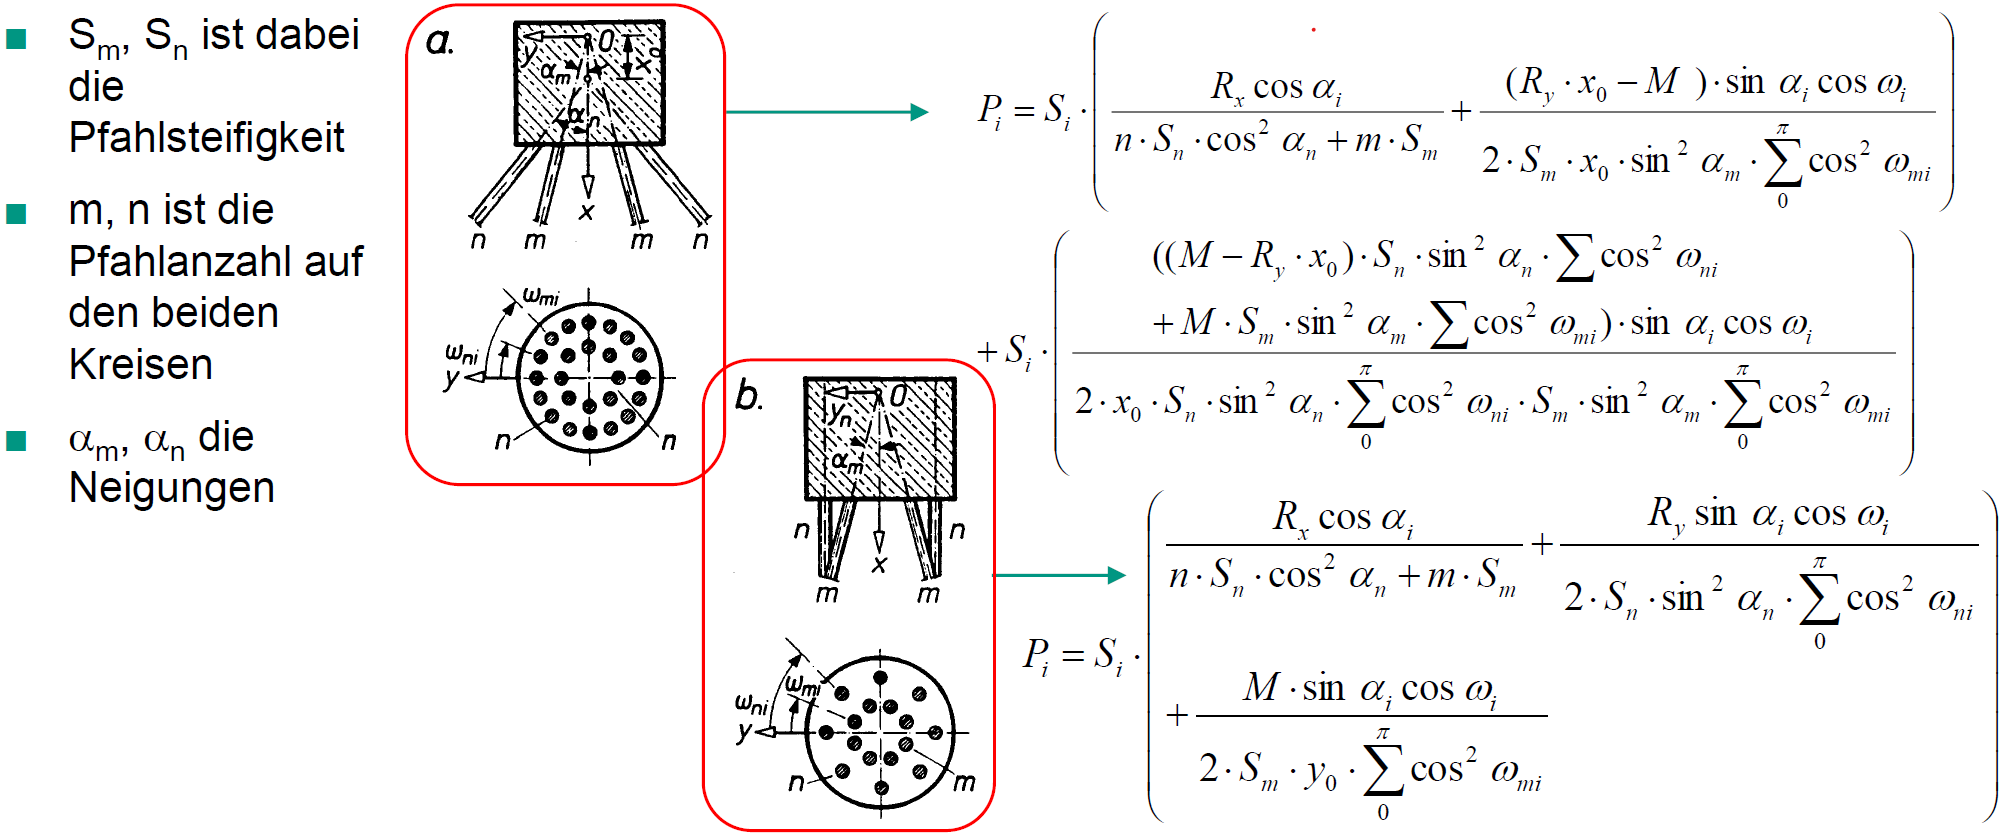
\includegraphics[width=0.99\textwidth]{Grafiken/Rotsym_Pfahl.png}\\

\rule{\textwidth}{0.075cm}

\subsubsection{Verfahren mit \enquote{m-Formel} nach Culmann}
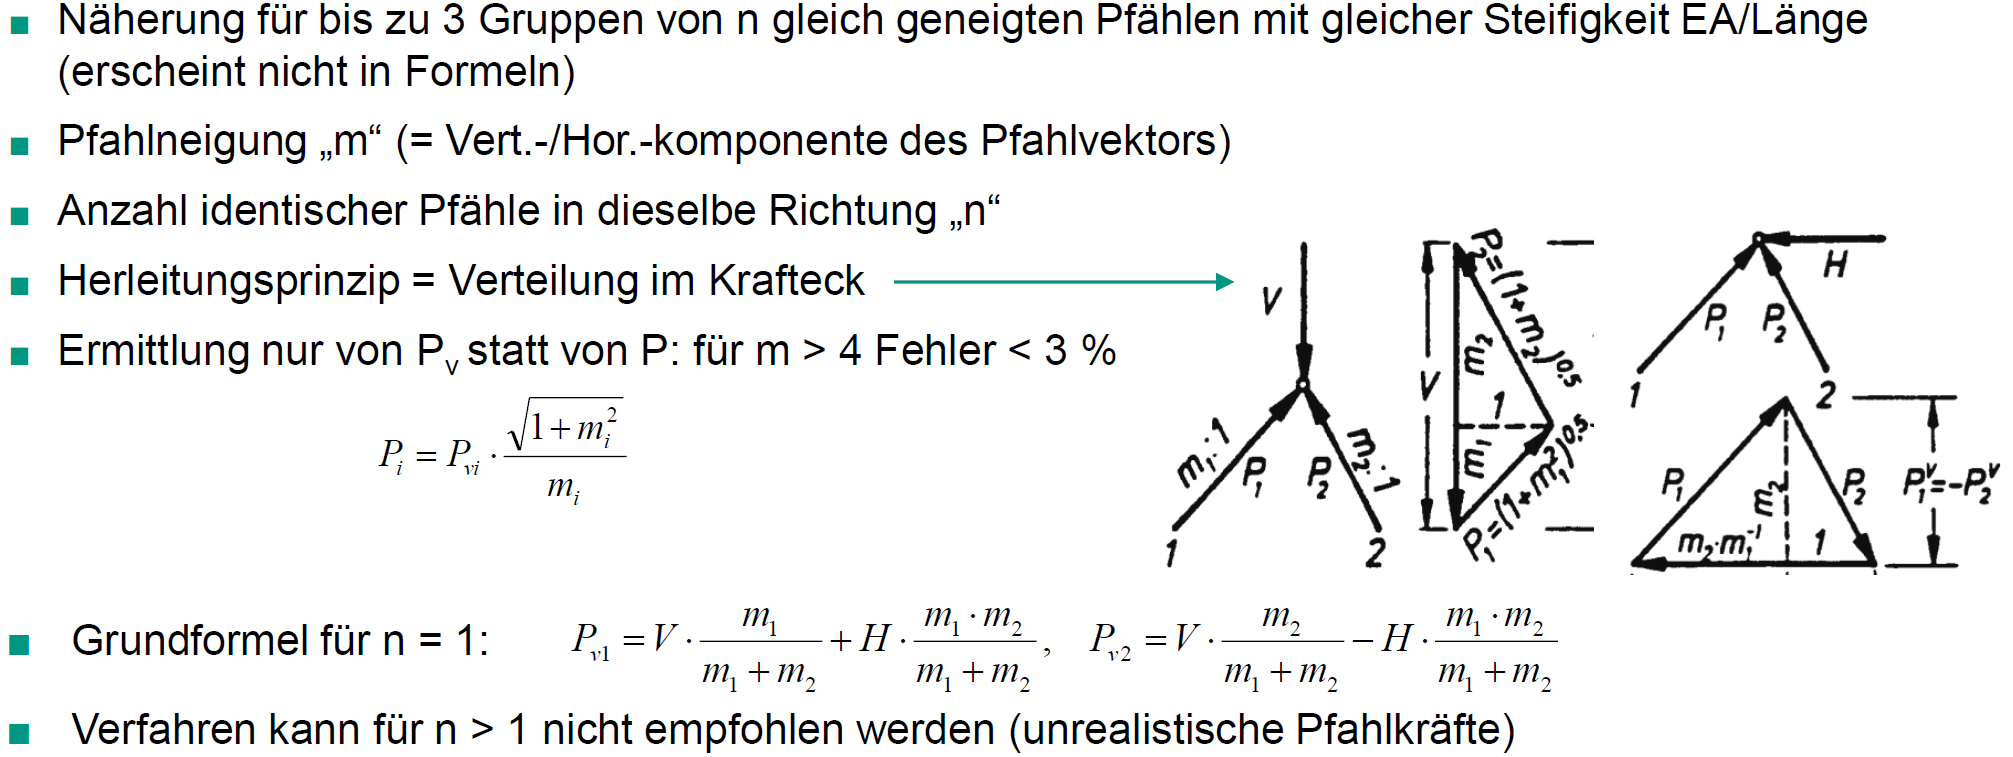
\includegraphics[width=0.99\textwidth]{Grafiken/Culmann_1.png}\\
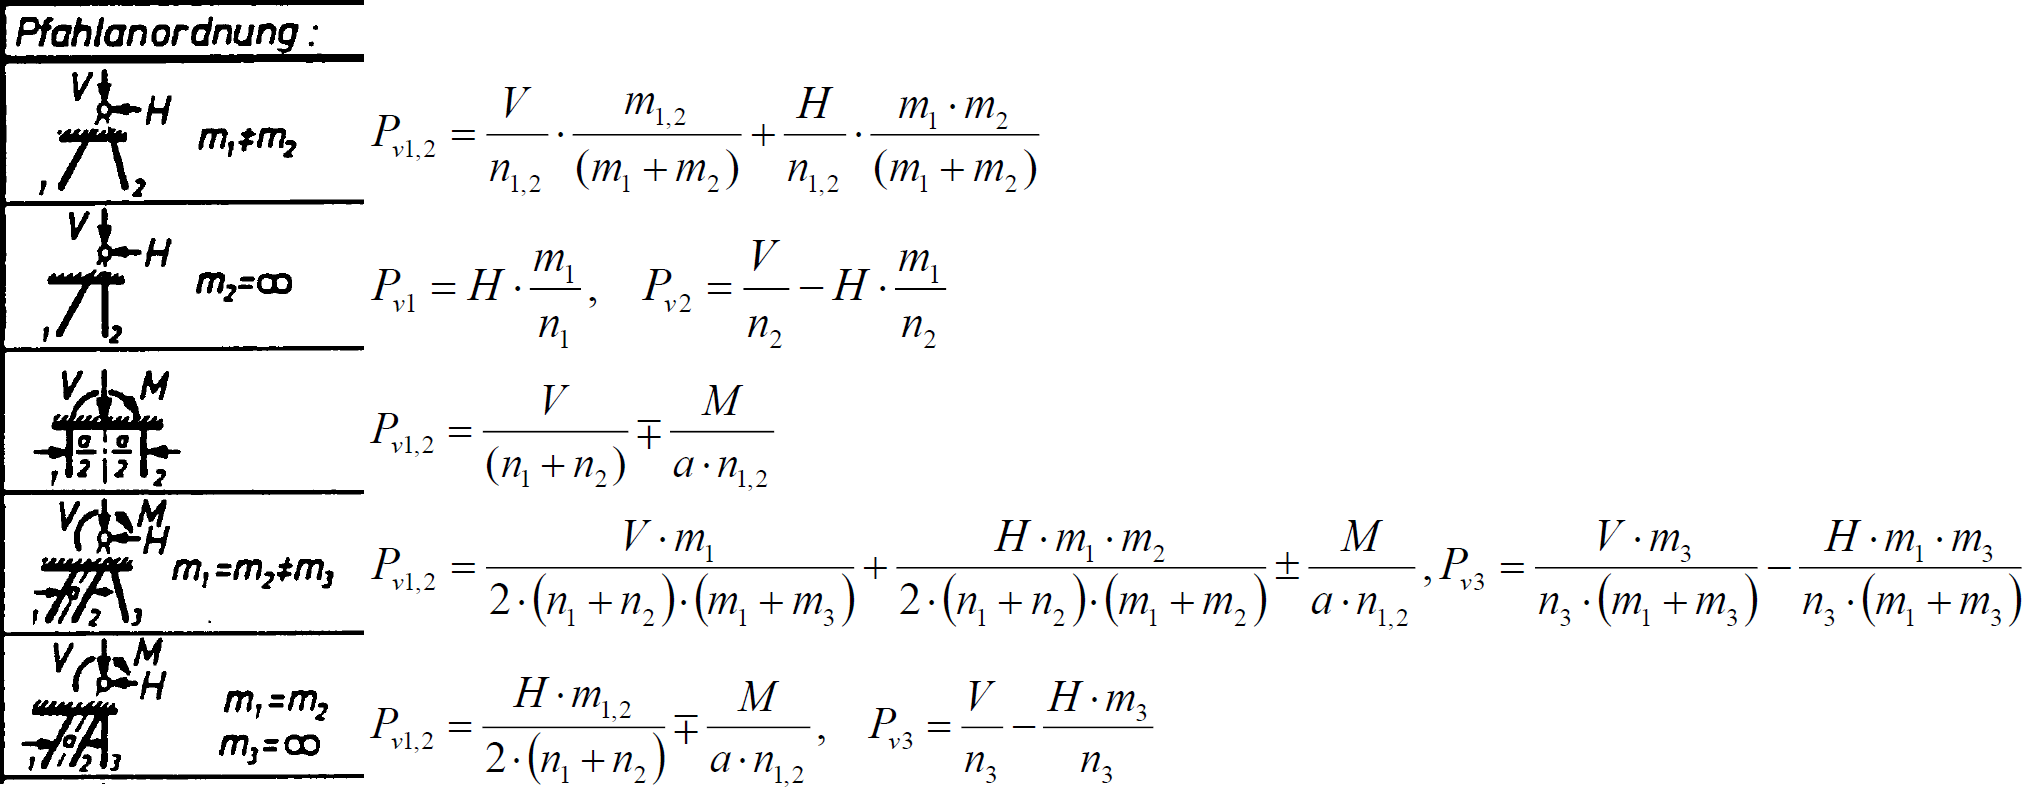
\includegraphics[width=0.99\textwidth]{Grafiken/Culmann_2.png}\\
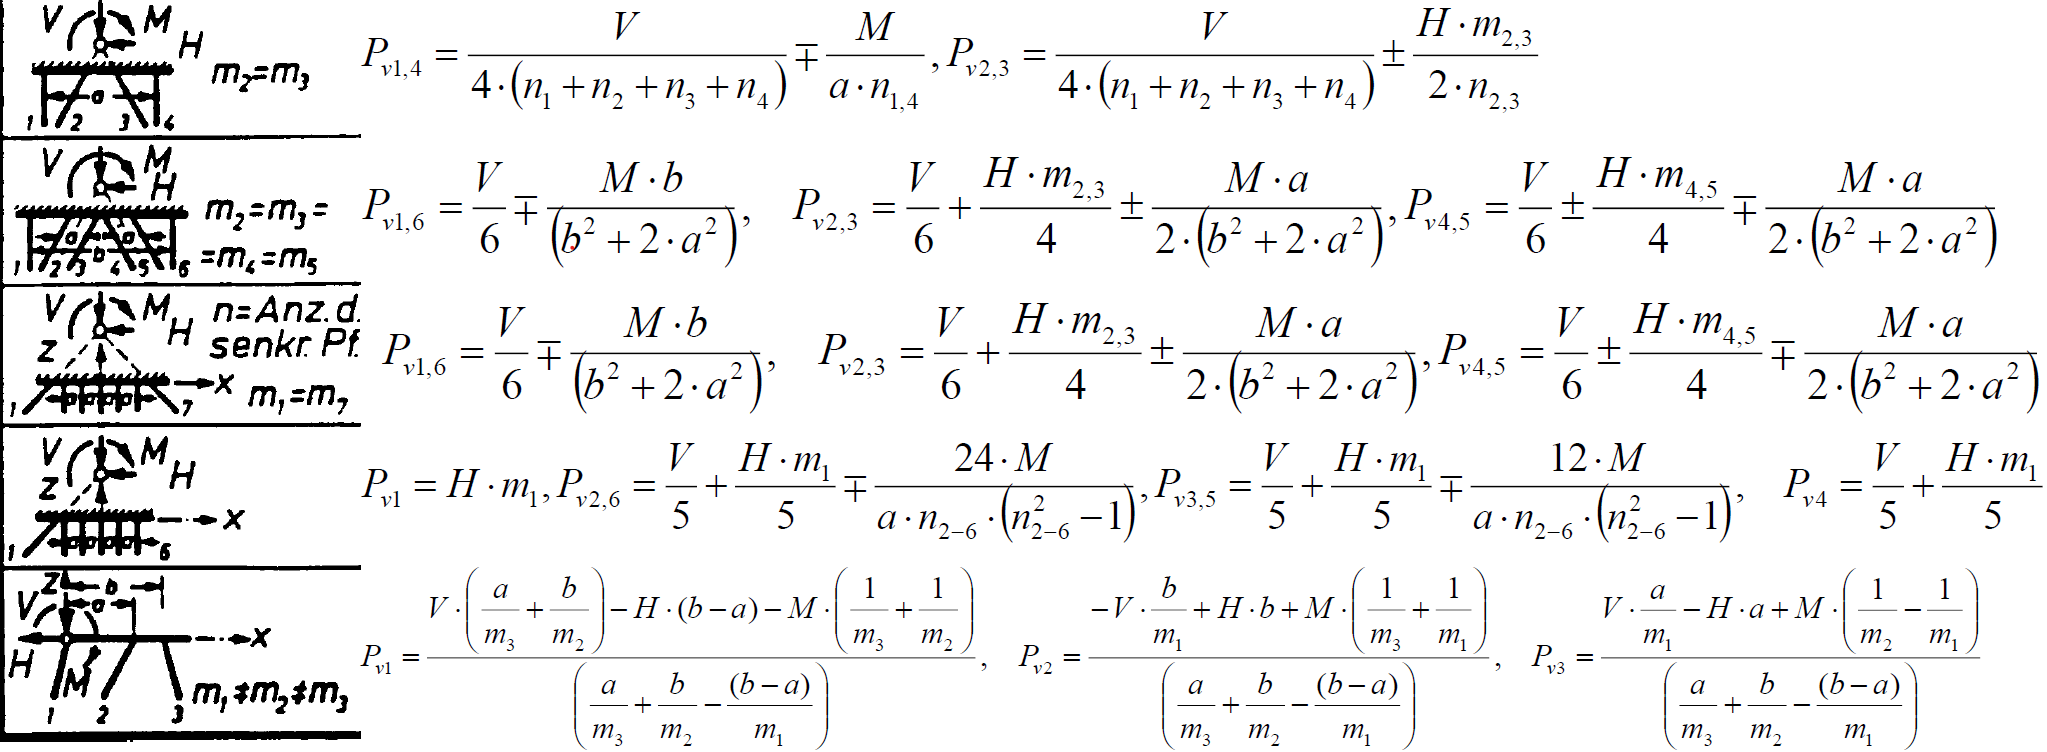
\includegraphics[width=0.99\textwidth]{Grafiken/Culmann_3.png}\\

\rule{\textwidth}{0.075cm}

\subsubsection{Verfahren nach Nökkentved}
\includegraphics[width=0.99\textwidth]{Grafiken/Nökkentved_1.png}\\
\includegraphics[width=0.99\textwidth]{Grafiken/Nökkentved_2.png}\\
\includegraphics[width=0.99\textwidth]{Grafiken/Nökkentved_3.png}\\
\includegraphics[width=0.99\textwidth]{Grafiken/Nökkentved_4.png}\\
\includegraphics[width=0.99\textwidth]{Grafiken/Nökkentved_5.png}\\
\includegraphics[width=0.99\textwidth]{Grafiken/Nökkentved_6.png}\\
\includegraphics[width=0.99\textwidth]{Grafiken/Nökkentved_7.png}\\
\rule{\textwidth}{0.075cm}

\subsection{Setzungsberechnung}

\begin{itemize}
    \item Starre Kopfplatte
    \begin{enumerate}
        \item Vorgabe Pfahlanzahl $n$ und Geometrie $a/d$
        \item Ermittlung Tragfähigkeit Einzelpfahl $R_{E,s=0,1D}$ für Grenzsetung $s_E=0,1D$
        \item Ermittlung von $\lambda_1$, $\lambda_2$, $\lambda_3$ und damit Tragfähigkeit $R_{G,i,s=0,1D}=R_{E,s=0,1D}\cdot G_{R,i}$ der Einzelpfähle je nach Position, $G_{R,i}=\lambda_1\cdot\lambda_2\cdot\lambda_3$
        \item Summation aller $R_{G,i,s=0,1D}$
        \item Bestimmung Ausnutzungsgrad $\frac{F_G}{n_G\cdot R_{G,i,s=0,1D}}$ Gegenüber äußerer Einwirkung $F_G$
        \item Ermittlung von $S_1$ $S_2$, $S_3$ und Gruppenfaktor $G_S=S_1\cdot S_2\cdot S_3$
        \item Berechnung der \enquote{neuen} Setzung $s_G=G_S\cdot s_E$
        \item Iterieren bis Ausnutzungsgrad konvergiert
    \end{enumerate}
    \item Tiefergelegte Flachgründung:
    \begin{itemize}
        \item Ersatzebene in Höhe des Pfahlfußes: $B_G'=B_G+2\cdot3\cdot D_s$
        \item Setzungsberechnung nach Steinbrenner:
        \begin{itemize}
            \item Mittelpunkt der Gründungsfläche: $s_k=4\Delta p\cdot b\cdot f_s\frac{1}{E_s}$
        \end{itemize}
        \begin{itemize}
            \item Eckpunkt der Gründungsfläche: $s_k=\Delta p\cdot b\cdot f_s\frac{1}{E_s}$
        \end{itemize}
        \item Starre Kopfplatte: $s_{k,\text{starr}}=0,75\cdot s_{k,1/4}$
       \item Wenn: $\frac{6(E_{\text{Platte}I_{\text{Platte})\cdot l_{\text{Pfahl}}}}}{(E_{\text{Pfahl}}A_{\text{Pfahl}})\cdot a^3}>50$
    \end{itemize}
\end{itemize}

%\newpage
\section{Mess- und Kontrollverfahren}


\subsection{Messtechnische Überwachung von Stützkonstruktionen}
\begin{itemize}
    \item Kraftmessdosen: In allen Lagen an maßgebenden Punkten zur Überwachung Steifenkraft
    \item Inklinometer: Hinter Schlitzwand etc. Evtl. Nullmessung zu Bestimmung Ausgangslage
    \item Hebungsmessung in Sohle
    \item Setzungsmessung im Gelände neben Baugrube
    \item Manometer: Porenwasserdruckmessung zur Bestimmung Pegel in Höhe Wandfuß
\end{itemize}


%\newpage
\section{Theoriefragen}

\begin{itemize}
    \item Wann wird bei Ansatz des ebenen Erdrucks die Wandreibung überschätzt?\\
    $\blacktriangleright$ $\frac{H}{r} \geq 2,0$ $\Rightarrow$ Radiale Verspannung des Bodens reduziert den aktiven Erddruck. Bei unnachgiebiger Wand wird der (Ruhe-)druck gegenüber dem ebenen Fall nicht reduziert.
    \item Aushub nach Herstellung Bohrpfähle (mit Leerbohrstrecke von Voraushubniveau). Warum Zugkraft weiterer Aushub?\\
        $\blacktriangleright$ Durch die Entlastungshebung der BGS erfahren sie eine Längung und durch die spätere Druckbelastung eine Lastumkehr (unvermeidlich). Gefahr einer Überlastung (Zwangskraft inf. Längung plus Auftrieb Pfahlkopfplatte) besteht nicht, wenn die Sohle Pfahlkopfplatte bis zum Erreichen des Bauwerksgewichts dräniert bleibt.
    \item Zulässigen Bemessungsverfahren für eine KPP und beschreiben Sie den Nachweis der äußeren Tragfähigkeit (ULS). $\blacktriangledown$
        \begin{enumerate}
            \item Empirische Berechnungsverfahren
            \item Verfahren auf der Basis äquivalenter Ersatzmodelle (\enquote{equivalent raft method}, \enquote{equivalentpile method} u.a.)
            \item Analytische Berechnungsverfahren (Verfahren nach dem Prinzip der wegunabhängigen Stützung, Verfahren mit Superposition elastischer Setzungsanteile)
            \item Numerische Verfahren (FEM u.a.)
        \end{enumerate}
        Bei nicht rechteckigem Grundriss: allein Nr. 4.\\
        Äußere Tragfähigkeit aus Gesamtlast $S_{k,i}$ vs. Grundbruchwiderstand des eingeschlossenen Bodenblocks:\\
        $\sum \gamma_{S,i} \cdot S_{k,i} \leq \frac{\sum (R_{pile,j} + R_{raft} )}{\gamma_{R}} $
    \item Unterschied zwischen Graben- und Dammbedingung\\
        $\blacktriangleright$ Grabenbedingung: Verfüllung in vergleichsweise engem Schlot zwischen Böschung und Bauwerk, Verfüllboden hängt sich an Grabenwänden auf und bildet ein Gewölbe $\Rightarrow$ reduzierte Auflast auf Rahmenbauwerk.\\
        $\blacktriangleright$ Dammbedingung: Rahmenbauwerk bildet über nennenswerten Teil der Verfüllhöhe eine steifere Struktur als Verfüllboden, Verfüllboden hängt sich Bauwerkswänden auf $\blacktriangleright$ erhöhte Auflast auf Rahmenbauwerk.
    \item Erdstatischen Ansätzen für gebettetes Rahmentragwerk mit variablem Radius (Maulquerschnitt) bemessen? Wie erhält man die maßgebende Bettungsziffer?
        \begin{itemize}[label=$\blacktriangleright$]
            \item Elastisch gebettete Gelenkkette, Firste auf 45° bettungsfrei
            \item Belastung aus Überlagerungsgewicht, Erddruck und Wasserdruck (Endzustand)
            \item Radiale Bettung mit dem lokalen Radius R und der Steifeziffer des Bodens, C $\approx$ 1: $k_r = D\cdot \frac{E_s}{R}$\\
            Ggf. auch tangentiale Bettung (Schnittkraftreduktion)
        \end{itemize} 
    \item Warum hat die Nachgiebigkeit (Geotextilmatte) oder Rauhigkeit (Abdichtungsfolie) der \\Rahmenaußenfläche Konsequenzen für die Schnittkraftverteilung?
        \begin{itemize}[label=$\blacktriangleright$]
            \item Nachgiebigkeit bedeutet kleinere radiale Bettungsziffer $\Rightarrow$ höhere Schnittkräfte
            \item Glatte Außenhaut bedeutet keine tangentiale Bettung $\Rightarrow$ höhere Schnittkräfte
        \end{itemize} 
    \item Techniken und Bauhilfsmaßnahmen unterfahren eines rechteckigen Stahlbetonrahmen die Bahnstrecke auch unter Betrieb
        \begin{enumerate}
            \item Ggf. verbaute und abgedichtete Trogbaugrube beidseits des Gleises (hier durch Graben und GWA schon gegeben)
            \item Widerlagerwand in Baugrube
            \item Rahmenquerschnitt mit Schneide auf Verschubbahn komplett aufbetonieren
            \item Ca. 1 m dicke Frostplatte unter dem Gleis mit Stickstoff in horizontal eingebohrtem Lanzenschirm gefrieren
            \item Gleis über Kleinhilfsbrücken und Verschubträger auf Frostkörper und Schneidenträger auflagern
            \item Engmaschige Gleislagenüberwachung, Langsamfahrstrecke
            \item Rahmenquerschnitt mit hydr. Pressen gegen Bahndamm verschieben, Bahndamm sukzessive abbaggern und Frostdeckel sprengen
        \end{enumerate}
    \item Berechnungsverfahren zur Ermittlung der Schnittkräfte aus der statischen Last einer Zugüberfahrt anzuwenden, wenn unterhalb der Schottertragsch:
        \begin{enumerate}[label=(\alph*)]
            \item inkompressibler Fels\\
            $\blacktriangleright$ Die Schottertragschicht stellt eine \enquote{Matratze} begrenzter Dicke dar; das Bettungsmodulverfahren kann verwendet werden. $\Rightarrow$ Block-Feder Modell.
            \item eine verdichtete Auffüllung mit ähnlicher Steifigkeit wie die Schottertragschicht ansteht?\\
            $\blacktriangleright$ Unterhalb der Festen Fahrbahn existiert ein elastischer Halbraum; das Steifemodulverfahren ist anzuwenden $\Rightarrow$ elastisches Kontinuum
        \end{enumerate}

    \item \textbf{Geotechnische Kategorien:}
        \begin{itemize}
            \item Allgemeines:\\
                In DIN 1054 werden für die drei Geotechnischen Kategorien 1, 2, 3 die Kurzzeichen GK 1, GK 2, GK 3 verwendet.
                Die Einstufung in die Geotechnischen Kategorien GK 1, GK 2 oder GK 3 ist vor Beginn der geotechnischen Erkundung unter Beachtung der nachfolgenden Regeln und jener von DIN 4020 vorzunehmen. Maßgebend für die Einstufung ist jenes Kriterium, das die höchste Geotechnische Kategorie ergibt. Die Einstufung und die daraus resultierenden Anforderungen sind im Zuge der Projektbearbeitung aufgrund der Ergebnisse geotechnischer Untersuchungen, Berechnungen und der Bauausführung zu überprüfen und gegebenenfalls anzupassen.\vspace*{8pt}\\
                $\blacktriangleright$ GK1: Baumaßnahmen mit geringem Schwierigkeitsgrad im Hinblick auf Bauwerk und Baugrund.
                    \begin{itemize}
                    \item Die Geotechnische Kategorie GK 1 setzt einfache und überschaubare Baugrundverhältnisse voraus.
                        Gegebenheiten, die diese Einstufung rechtfertigen, liegen vor, wenn der Baugrund in waagerechtem oder
                        schwach geneigtem Gelände nach gesicherter örtlicher Erfahrung als tragfähig und setzungsarm bekannt ist.
                    \item Die Einstufung in die Geotechnische Kategorie GK 1 setzt voraus, dass Grundwasser unterhalb der
                        Baugruben- bzw. Gründungssohle liegt.
                    \item Gegebenheiten des Bauwerks, die eine Einstufung in die Geotechnische Kategorie GK 1 rechtfertigen, liegen in der Regel vor, wenn folgende Voraussetzungen erfüllt sind:
                        \begin{itemize}
                            \item es handelt sich um setzungsunempfindliche, flach gegründete Bauwerke mit Stützenlasten bis 250 kN
                            und Streifenlasten bis 100 kN/m wie Einfamilienhäuser, eingeschossige Hallen, Garagen;
                            \item es handelt sich um Bauwerke, bei denen nach DIN EN 1998-5/NA im Hinblick auf Erdbebenbelastung
                            kein Nachweis der Standsicherheit erforderlich ist;
                            \item Nachbargebäude, Verkehrswege, Leitungen usw. werden durch das Bauwerk selbst oder durch die für
                            seine Errichtung notwendigen Bauarbeiten nicht in ihrer Standsicherheit gefährdet oder in ihrer                Gebrauchstauglichkeit beeinträchtigt.
                        \end{itemize}
                    \end{itemize}
                $\blacktriangleright$ GK2: Baumaßnahmen mit mittlerem Schwierigkeitsgrad im Hinblick auf das Zusammenwirken von Bauwerk und Baugrund.
                    \begin{itemize}
                        \item Bauwerke der Geotechnischen Kategorie GK 2 erfordern eine ingenieurmäßige Bearbeitung und
                einen rechnerischen Nachweis der Standsicherheit und der Gebrauchstauglichkeit.
                        \item Die Geotechnische Kategorie GK 2 setzt durchschnittliche Baugrundverhältnisse voraus, die nicht in
                GK 1 oder GK 3 fallen.
                        \item Die Geotechnische Kategorie GK 2 setzt durchschnittliche Grundwasserverhältnisse voraus.
                Beispiele dafür sind:
                            \begin{itemize}
                                \item die freie Grundwasseroberfläche liegt höher als die Bauwerkssohle;
                                \item Grundwasserzutritte bzw. die Wasserhaltung sind mit üblichen Maßnahmen beherrschbar;
                                \item durch diese Maßnahmen sind keine ungünstigen Einflüsse auf die Umgebung zu befürchten.
                            \end{itemize}
                        \item Zur Geotechnischen Kategorie GK 2 gehören:
                            \begin{itemize}
                                \item übliche Hoch- und Ingenieurbauten auf Einzelfundamenten, Streifenfundamenten, Gründungsplatten                 oder auf Pfahlgründungen;
                                \item Leitungsgräben bis 5 m Tiefe;
                                \item Bauwerke der Bedeutungskategorien I und II nach DIN EN 1998-5/NA, bei denen im Hinblick auf                 Erdbebenbelastung ein Nachweis der Standsicherheit erforderlich ist;
                                \item Bauvorhaben, bei denen durch konstruktive Maßnahmen, z. B. dichte und steife                 Baugrubenumschließung, ein schädlicher Einfluss der Baumaßnahme auf Nachbarschaft und Umgebung                 nicht zu erwarten ist.
                            \end{itemize}
                        \item In der Regel dürfen auch besondere Bauwerke wie unterirdisch aufgefahrene Hohlraumbauten, Tunnel, Stollen und Schächte in festem, wenig geklüftetem Fels der Geotechnischen Kategorie GK 2 zugeordnet werden.
                        \item Als sonstige Baumaßnahmen zählen in der Regel zur Geotechnischen Kategorie GK 2 auch
                            \begin{itemize}
                                \item Boden- und Felsdeponien ohne Kontamination und
                                \item übliche Horizontalbohrungen für den Leitungsbau.
                            \end{itemize}
                    \end{itemize}
                $\blacktriangleright$ GK3: Bauwerke der Geotechnischen Kategorie GK 3 erfordern über die Vorgaben von GK2 zusätzliche Untersuchungen sowie vertiefte geotechnische Kenntnisse und Erfahrungen in dem jeweiligen Spezialgebiet.
                    \begin{itemize}
                        \item Die Geotechnische Kategorie GK 3 umfasst Baumaßnahmen mit hohem Schwierigkeitsgrad im Hinblick auf das Zusammenwirken von Bauwerk und Baugrund.
                        \item Gegebenheiten des Baugrunds, die in der Regel eine Einstufung in die GK 3 erfordern, sind ungewöhnliche oder besonders schwierige Baugrundverhältnisse wie:
                            \begin{itemize}
                                \item geologisch junge Ablagerungen mit regelloser Schichtung bzw. geologisch wechselhafte Formationen;
                                \item Böden, die zum Kriechen, Fließen, Quellen oder Schrumpfen neigen;
                                \item bindige Böden, bei denen die Restscherfestigkeit maßgebend sein kann;
                                \item bindige Böden ohne ausreichende Duktilität, z. B. strukturempfindliche Seetone;
                                \item weiche organische und organogene Böden größerer Mächtigkeit;
                                \item Fels, der zur Auflösung oder zu starkem Zerfall neigt, z. B. Salz, Gips und verschiedene veränderlich feste Gesteine;
                                \item Fels, der in Bezug auf das Bauvorhaben ungünstig verlaufende Störungszonen oder Trennflächen
                                enthält;
                                \item Bergsenkungsgebiete oder Gebiete mit Erdfällen oder Baugrund mit ungesicherten Hohlräumen;
                                \item unkontrolliert geschüttete Auffüllungen.
                            \end{itemize}
                        \item Gespanntes Grundwasser, das durch Bodenaushub zu artesischem Grundwasser werden kann, ist der              Geotechnischen Kategorie GK 3 zuzuordnen.
                        \item Ergänzend werden als Beispiele für Bauwerke der Geotechnischen Kategorie GK 3 genannt:
                            \begin{itemize}
                                \item Bauwerke mit hohem Sicherheitsanspruch oder hoher Verformungsempfindlichkeit;
                                \item Bauwerke mit ungewöhnlichen Lastkombinationen, die für die Gründung maßgebend werden;
                                \item Bauwerke, die durch Wasser mit einer Druckhöhe von mehr als 5 m belastet sind;
                                \item Einrichtungen und Baumaßnahmen, die den Grundwasserspiegel vorübergehend oder bleibend                verändern, sofern damit ein Risiko für benachbarte Bauten entsteht;
                                \item Bauwerke der Bedeutungskategorien III und IV nach DIN EN 1998-5/NA, bei denen im Hinblick auf                Erdbebenbelastung ein Nachweis der Standsicherheit erforderlich ist;
                                \item Bauwerke oder Baumaßnahmen, bei denen die Beobachtungsmethode zum Nachweis der Standsicherheit und der Gebrauchstauglichkeit angewendet wird.
                            \end{itemize}
                        \item Als besondere Bauwerke zählen in der Regel zur Geotechnischen Kategorie GK 3 auch:
                            \begin{itemize}
                                \item Senkkastengründungen mit Druckluft;
                                \item unterirdisch aufgefahrene Hohlraumbauten, Tunnel, Stollen und Schächte in Lockergestein oder in                geklüftetem Fels;
                                \item Kerntechnische Anlagen;
                                \item Offshore-Bauten;
                                \item Chemiewerke und Anlagen, in denen gefährliche chemische Stoffe erzeugt, gelagert oder umgeschlagen                werden.
                            \end{itemize}
                        \item Als sonstige Baumaßnahmen zählen in der Regel zur Geotechnischen Kategorie GK 3 auch:
                            \begin{itemize}
                                \item Deponien aller Art, ausgenommen nicht kontaminierte Böden und Felsaushübe;
                                \item Horizontalbohrungen mit hohen Spülungsdrücken z. B. im HDD-Verfahren (Horizontal Direction                Drilling), Microtunneling;
                                \item Verfahren des Spezialtiefbaus wie Schlitzwände, Einpressarbeiten und Düsenstrahlarbeiten.
                            \end{itemize}
                    \end{itemize}
        \end{itemize}
    
\end{itemize}

\end{document}
